\documentclass[12pt,letterpaper]{article}

\usepackage[utf8]{inputenc}
\usepackage[T1]{fontenc}
\usepackage{amsmath}
\usepackage{amsfonts}
\usepackage{amssymb}
\usepackage{amsthm}
\usepackage[left=2cm,right=2cm,top=2cm,bottom=2cm,headheight=22pt]{geometry}
\usepackage{fancyhdr}
\usepackage{setspace}
\usepackage{lastpage}
\usepackage{graphicx}
\usepackage{caption}
\usepackage{subcaption}


\theoremstyle{definition}
\newtheorem{question}{Question}
\newtheorem{example}{Example}
\newtheorem{exercise}[question]{Exercise}
\newtheorem*{challenge}{Challenge}

\begin{document}

%Paramètres de mise en forme des paragraphes selon les normes françaises
\setlength{\parskip}{1ex plus 0.5ex minus 0.2ex}
\setlength{\parindent}{0pt}

%Paramètres relatifs aux en-têtes et pieds de page.
\pagestyle{fancy}
\lhead{Theron J Hitchman}
\chead{\Large Images for Meeting 09}
\rhead{Fall 2013}
\lfoot{\emph{Math and Decision Making}}
\cfoot{}
\rfoot{\emph{\thepage\ of \pageref{LastPage}}}

\section*{Image for Question One: Is this knot tricolorable?}

\begin{figure}[h]
    \centering
    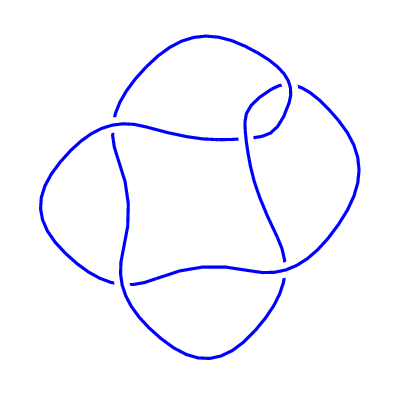
\includegraphics[width=.45\textwidth]{meeting09pics/5_2mirror.png}
    \caption{A knot with five crossings}
\end{figure}

\section*{Image for Question Two: Is this knot tricolorable?}

\begin{figure}[h]
    \centering
    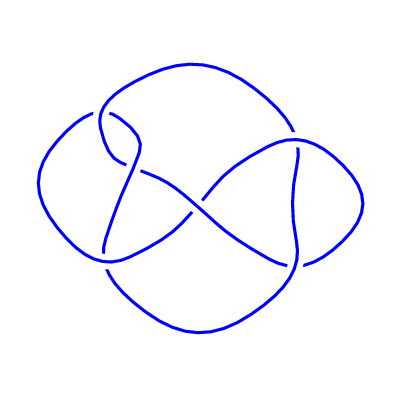
\includegraphics[width=.45\textwidth]{meeting09pics/6_3.png}
    \caption{A knot with six crossings}
\end{figure}

\clearpage

\section*{Image for Question One: Is this knot tricolorable?}

\begin{figure}[h]
    \centering
    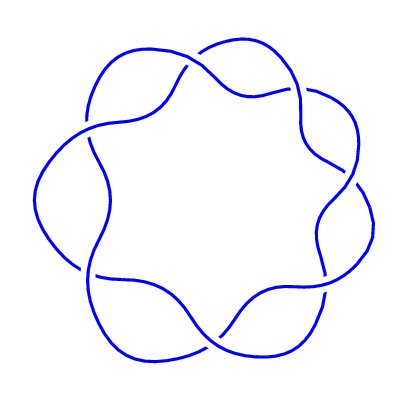
\includegraphics[width=.5\textwidth]{meeting09pics/7_1.png}
    \caption{A knot with seven crossings}
\end{figure}


\end{document}